\documentclass[a4paper, 10pt]{article}
\usepackage[utf8]{inputenc}
\usepackage[T1]{fontenc}
\usepackage[french]{babel}
\usepackage{graphicx}
\usepackage{listings}
\usepackage{amssymb}
\usepackage{amsmath}
\usepackage{fullpage}
\usepackage{url}
\usepackage[final]{pdfpages}

\begin{document}
\begin{center}
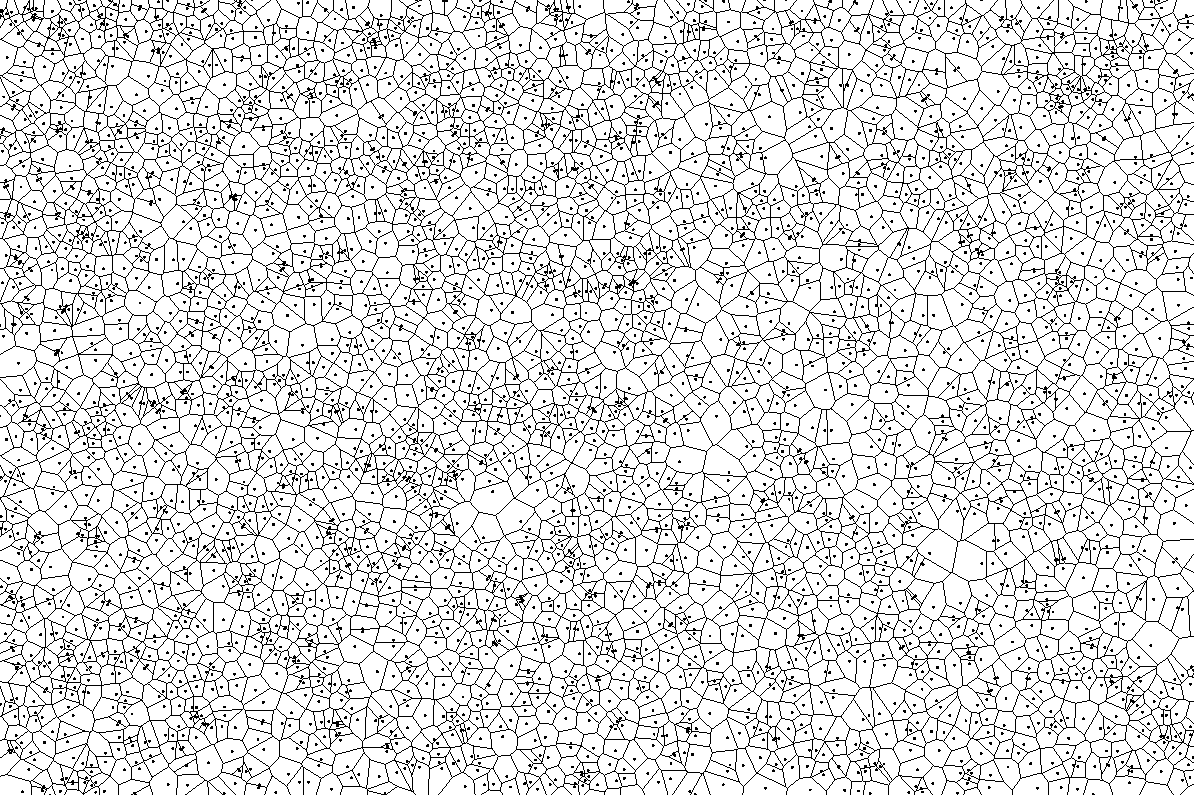
\includegraphics[scale=0.3]{Lloyd0.png}
  
\textbf{Figure 3}: diagramme de Voronoï d'un ensemble de 4000 points tirés au hasard.  
  
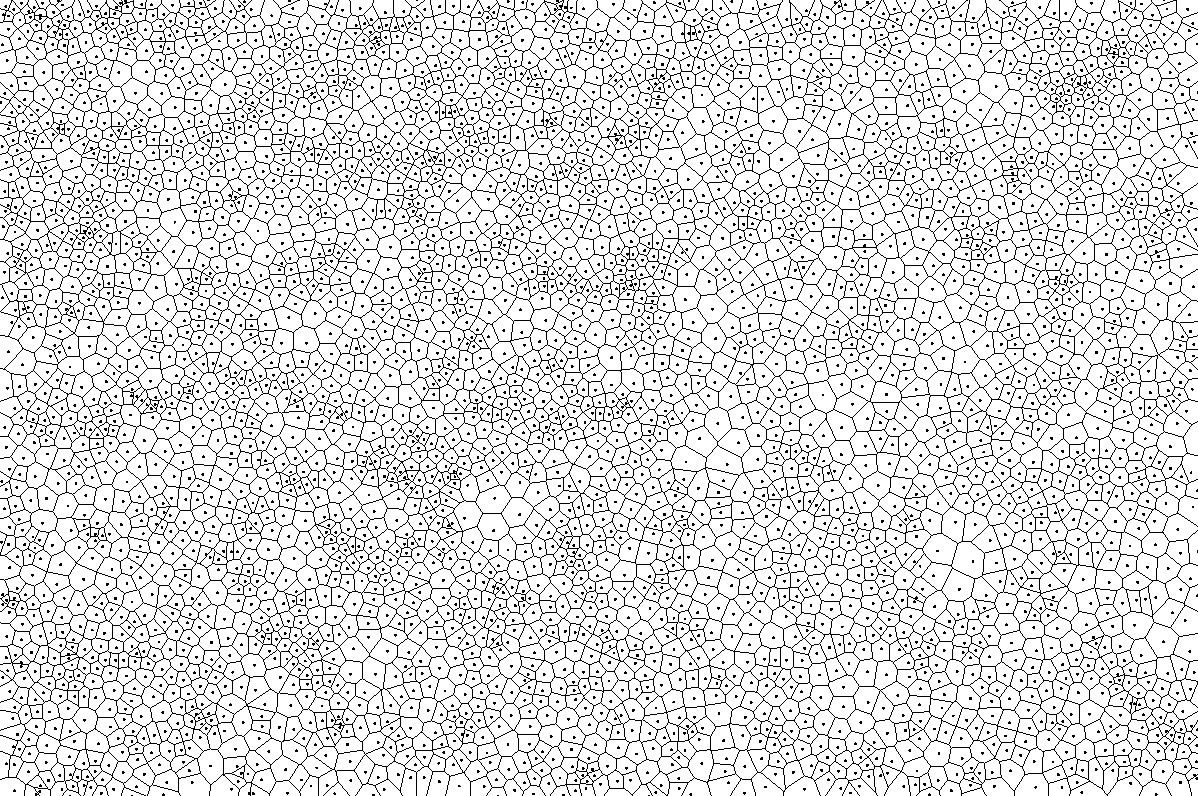
\includegraphics[scale=0.3]{Lloyd1.png}
  
\textbf{Figure 4}: même ensemble de points que \textbf{Figure 3}, après une itération de la relaxation de Lloyd.  
  
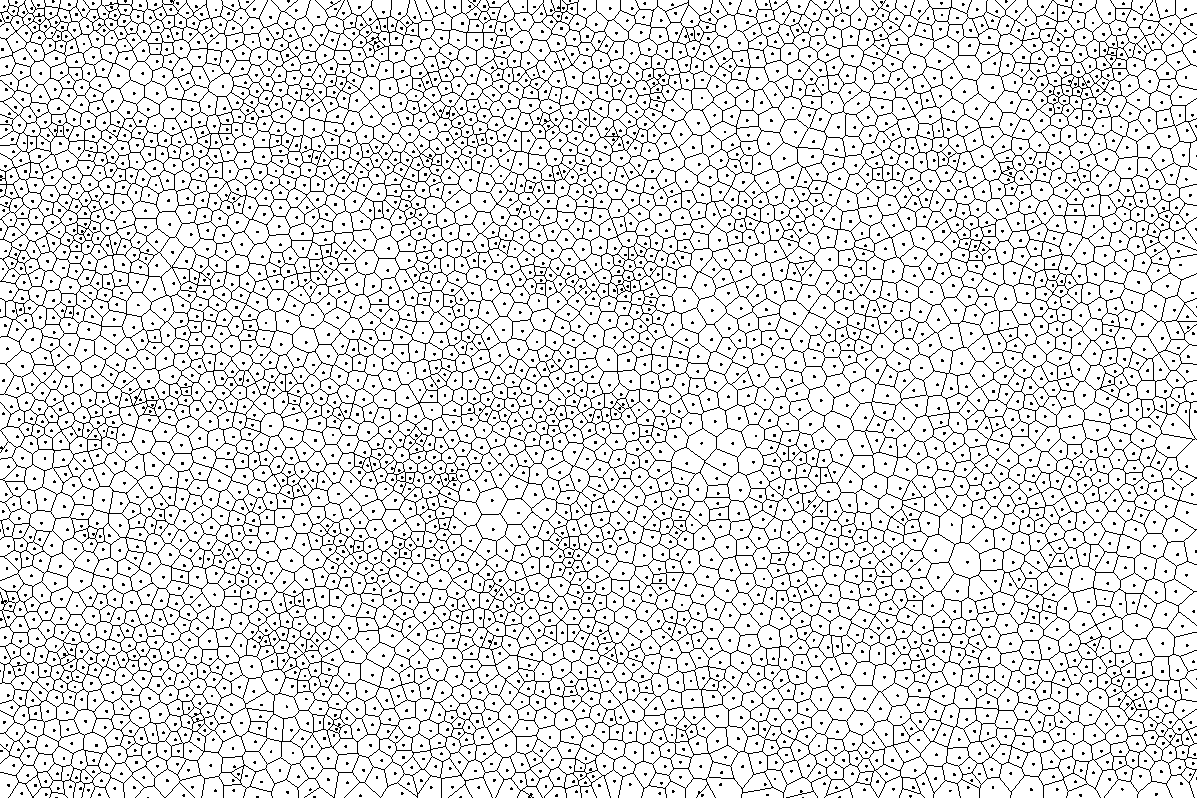
\includegraphics[scale=0.3]{Lloyd2.png}
  
\textbf{Figure 5}: même ensemble de points que \textbf{Figure 3}, après deux itérations de la relaxation de Lloyd. 
  
\newpage
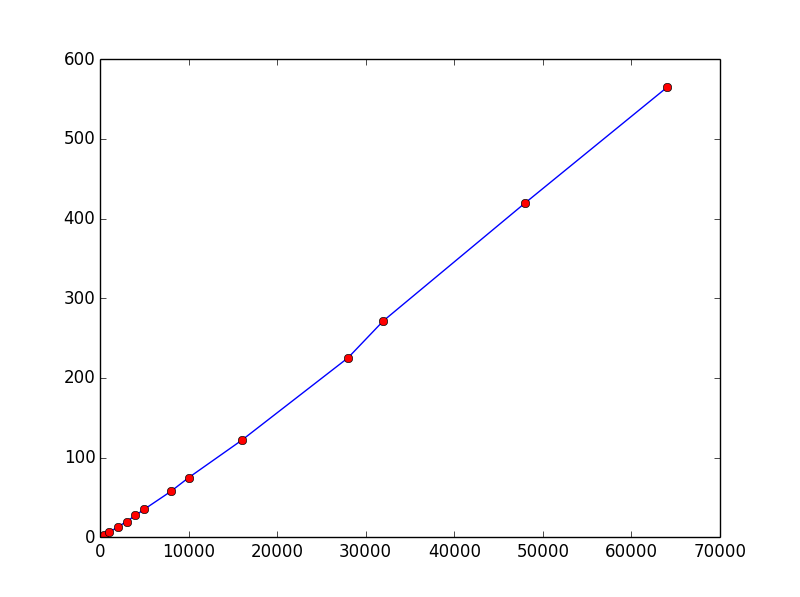
\includegraphics[scale=0.5]{PerformancesMilisecondes.png} 
  
\textbf{Figure 1}: nombre de sites en abscisse, et temps de calcul en ordonnée (en millisecondes) sur un Intel(R) Core(TM) i3-4010U CPU cadencé à 1.7GHz. Les temps pour les petits ensembles de points (inférieurs à 10 000) ont été moyennés sur plusieurs dizaines d'exécutions.  
  
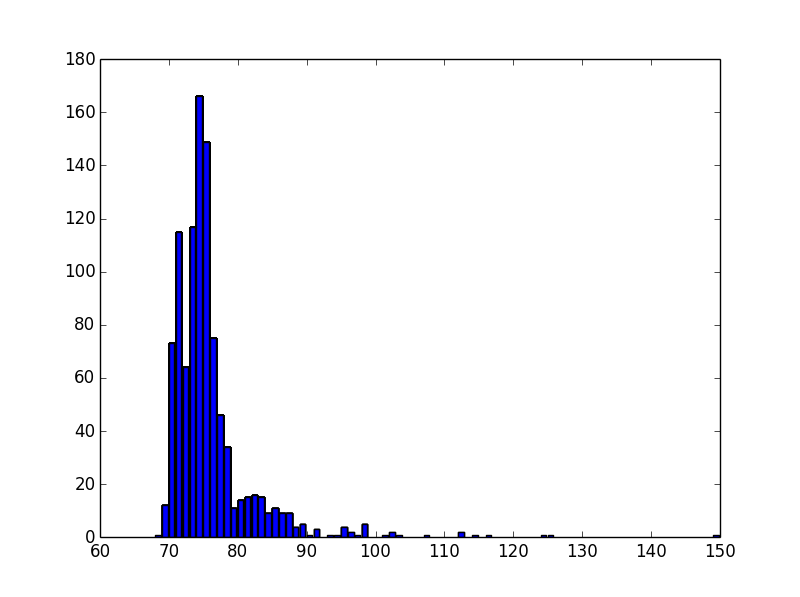
\includegraphics[scale=0.5]{PerformancesGaussienne.png}  
  
\textbf{Figure 2}: répartition des temps de calcul pour 1000 exécutions d'un ensemble de 10 000 points générés aléatoirement. En abscisse le temps de calcul (en millisecondes) et en ordonnée les effectifs. La courbe a l'allure d'une distribution à "queue épaisse". La plupart des temps se concentrent autour de la moyenne mais certains sont jusqu'à deux fois plus long.
  
\newpage
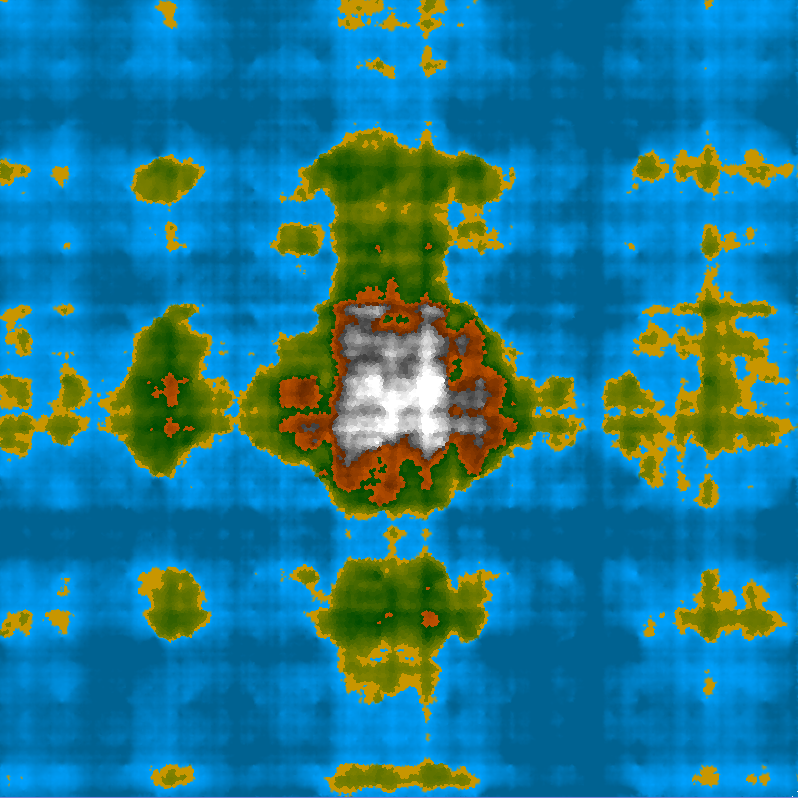
\includegraphics[scale=0.5]{GPUHash.png}  
  
\bigbreak   
\bigbreak 
\bigbreak 
  
    
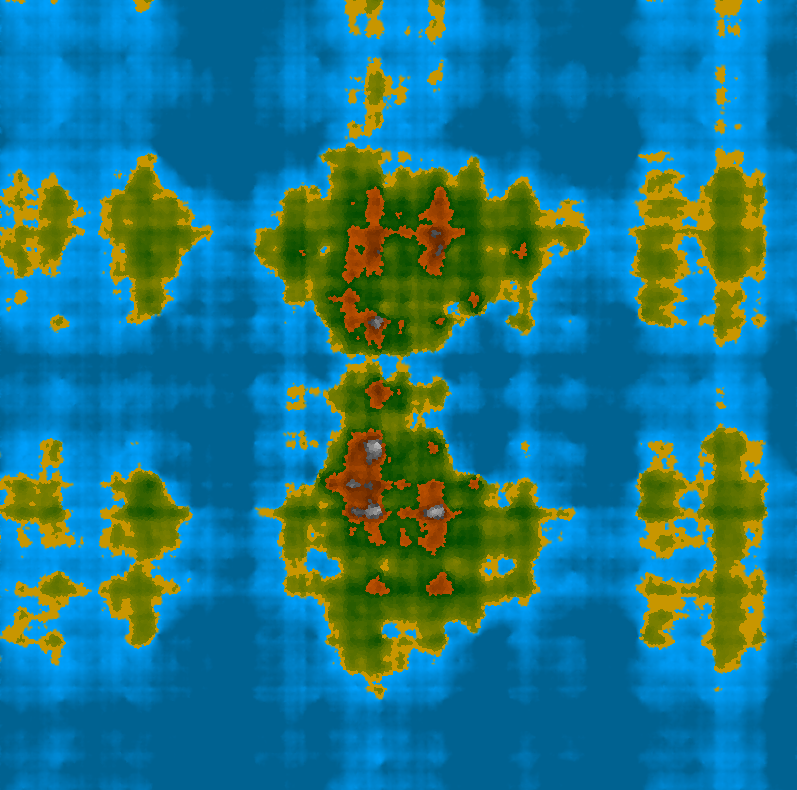
\includegraphics[scale=0.5]{GPUSymetrie.png}  

\end{center}
\end{document}
